\documentclass[12pt]{scrartcl}
\input{../styles/Packages.tex}
\input{../styles/FormatAndHeader.tex}

\setcounter{sheetnr}{3} % Nummer des Übungsblattes
\setcounter{exnum}{2} % Nummer der Aufgabe

% Beginn des eigentlichen Dokuments

\begin{document}

% Aufgabe 2
\exercise{Bonäre Suchbäume, AVL-Bäume}
  \begin{enumerate}
    \item Baum B2
      \begin{figure}[!h]
        \centering
        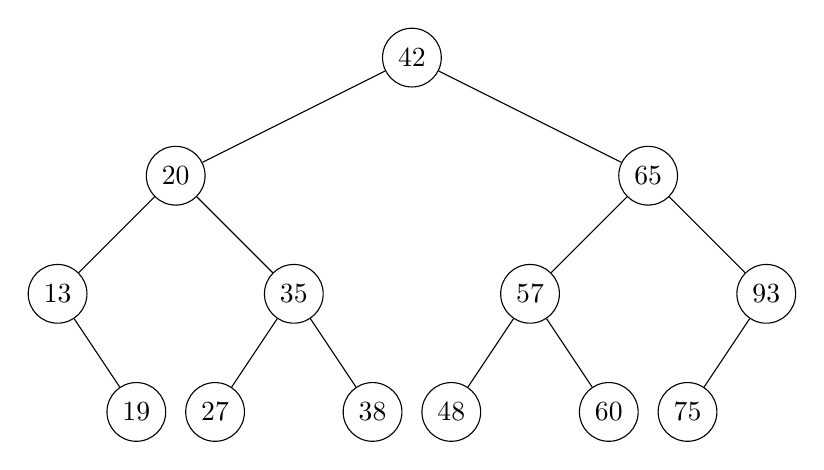
\begin{tikzpicture}[level/.style ={sibling distance=60mm/#1}]
          \node[circle,draw] (a) {42}
            child {node [circle,draw] (b) {20}
              child {node [circle,draw] (c) {13}
                child[missing] {node {}}
                child{node [circle, draw] (d) {19}}
              }
              child {node [circle, draw] (e) {35}
                child {node [circle, draw] (f) {27}}
                child {node [circle, draw] (g) {38}}
              }
            }
            child {node [circle, draw] (h) {65}
              child {node [circle, draw] (i) {57}
                child {node [circle, draw] (j) {48}}
                child {node [circle, draw] (k) {60}}
              }
              child {node [circle, draw] (l) {93}
                child {node [circle, draw] (m) {75}}
                child[missing] {node {}}
              }
            };
        \end{tikzpicture}
        \caption{Baum B2, indem B1 die Werte 19 und 60 eingefügt werden}
        \label{fig:baum}
      \end{figure}
    
    \item Baum B3
      \begin{figure}[!h]
        \centering
        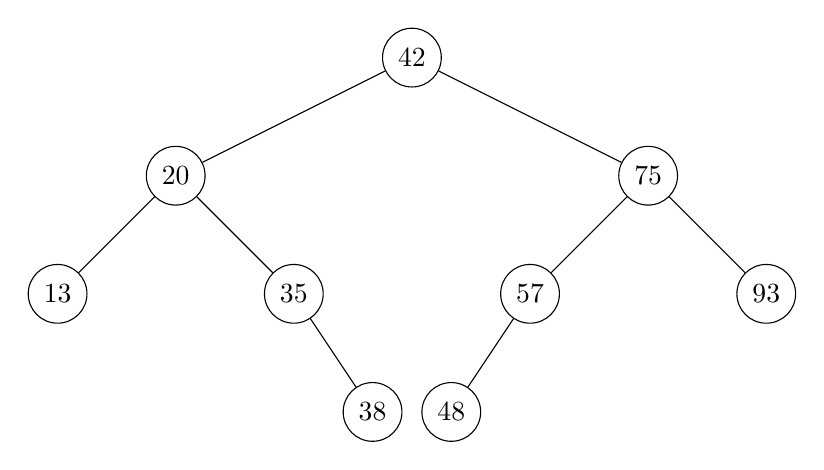
\begin{tikzpicture}[level/.style ={sibling distance=60mm/#1}]
          \node[circle,draw] (a) {42}
            child {node [circle,draw] (b) {20}
              child {node [circle,draw] (c) {13}}
              child {node [circle, draw] (e) {35}
                child[missing] {node {}}
                child {node [circle, draw] (g) {38}}
              }
            }
            child {node [circle, draw] (h) {75}
              child {node [circle, draw] (i) {57}
                child {node [circle, draw] (j) {48}}
                child[missing]{node{}}
              }
              child {node [circle, draw] (l) {93}}
            };
        \end{tikzpicture}
        \caption{Baum B3, indem aus B1 die Werte 27 und 65 entfernt werden}
        \label{fig:baum}
      \end{figure}
    
    \newpage

    \item B1 mit AVL-Balance
      \begin{figure}[!h]
        \centering
        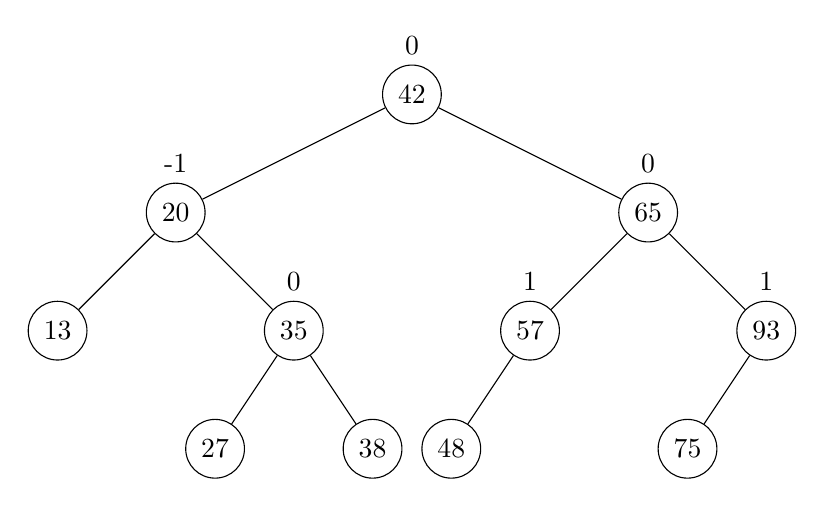
\begin{tikzpicture}[level/.style ={sibling distance=60mm/#1}]
          \node[circle,draw, label=0] (a) {42}
            child {node [circle,draw, label=-1] (b) {20}
              child {node [circle,draw] (c) {13}}
              child {node [circle, draw, label=0] (e) {35}
                child {node [circle, draw] (f) {27}}
                child {node [circle, draw] (g) {38}}
              }
            }
            child {node [circle, draw, label=0] (h) {65}
              child {node [circle, draw, label=1] (i) {57}
                child {node [circle, draw] (j) {48}}
                child[missing] {node {}}
              }
              child {node [circle, draw, label=1] (l) {93}
                child {node [circle, draw] (m) {75}}
                child[missing] {node {}}
              }
            };
        \end{tikzpicture}
        \caption{B1 mit AVL-Balance}
        \label{fig:baum}
      \end{figure}

    \item AVL-Baum
      \begin{enumerate}
        \item Baum B4(Ohne Reparierung)
          \begin{figure}[!h]
            \centering
            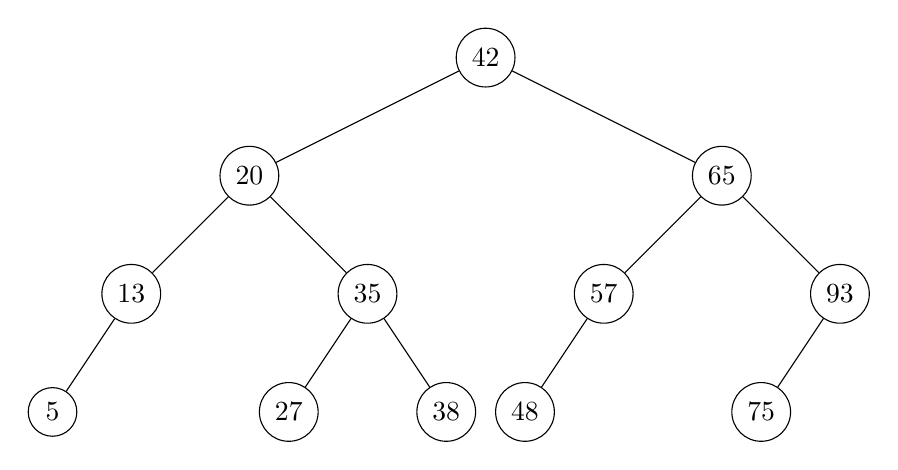
\begin{tikzpicture}[level/.style ={sibling distance=60mm/#1}]
              \node[circle,draw] (a) {42}
                child {node [circle,draw] (b) {20}
                  child {node [circle,draw] (c) {13}
                    child{node [circle, draw] (d) {5}}  
                    child[missing] {node {}}
                  }
                  child {node [circle, draw] (e) {35}
                    child {node [circle, draw] (f) {27}}
                    child {node [circle, draw] (g) {38}}
                  }
                }
                child {node [circle, draw] (h) {65}
                  child {node [circle, draw] (i) {57}
                    child {node [circle, draw] (j) {48}}
                    child[missing] {node {}}
                  }
                  child {node [circle, draw] (l) {93}
                    child {node [circle, draw] (m) {75}}
                    child[missing] {node {}}
                  }
                };
            \end{tikzpicture}
            \caption{Baum B4 durch Einfügen von 5 in B1}
            \label{fig:baum}
          \end{figure}
        
        \newpage 
        \item Baum B5(Rotation mit linkem Kind von 75 über 93 nach rechts)
          \begin{figure}[!h]
            \centering
            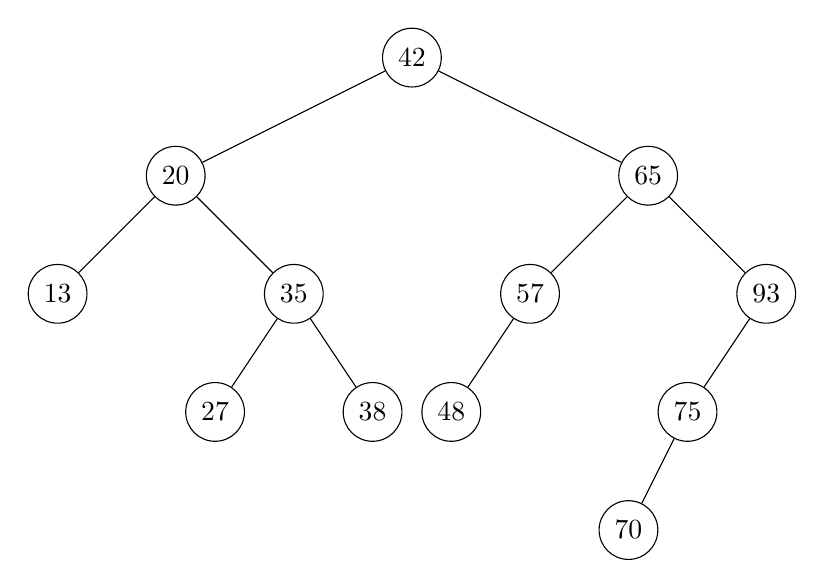
\begin{tikzpicture}[level/.style ={sibling distance=60mm/#1}]
              \node[circle,draw] (a) {42}
                child {node [circle,draw] (b) {20}
                  child {node [circle,draw] (c) {13}
                  }
                  child {node [circle, draw] (e) {35}
                    child {node [circle, draw] (f) {27}}
                    child {node [circle, draw] (g) {38}}
                  }
                }
                child {node [circle, draw] (h) {65}
                  child {node [circle, draw] (i) {57}
                    child {node [circle, draw] (j) {48}}
                    child[missing] {node {}}
                  }
                  child {node [circle, draw] (l) {93}
                    child {node [circle, draw] (m) {75}
                      child {node [circle, draw] (n) {70}}
                      child[missing] {node {}}
                    }
                    child[missing] {node {}}
                  }
                };
            \end{tikzpicture}
            \caption{Zwischenbaum: Baum B5 durch Einfügen von 70 in B1}
            \label{fig:baum}
          \end{figure}

          \begin{figure}[!h]
            \centering
            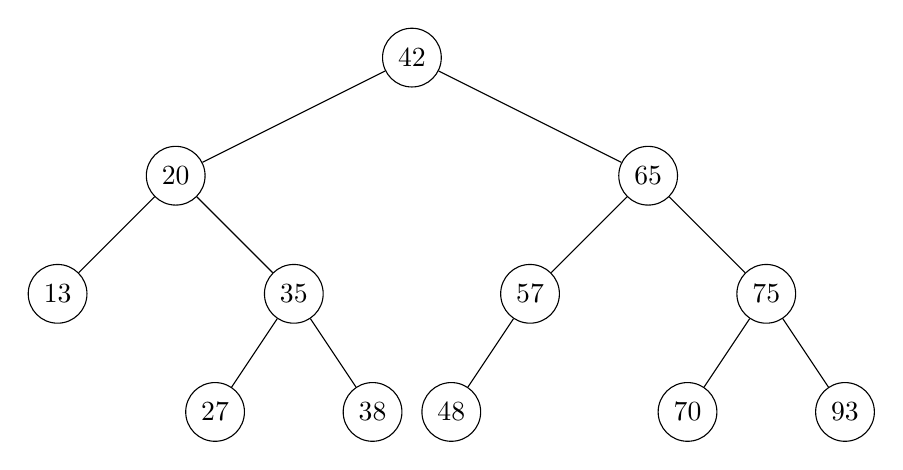
\begin{tikzpicture}[level/.style ={sibling distance=60mm/#1}]
              \node[circle,draw] (a) {42}
                child {node [circle,draw] (b) {20}
                  child {node [circle,draw] (c) {13}
                  }
                  child {node [circle, draw] (e) {35}
                    child {node [circle, draw] (f) {27}}
                    child {node [circle, draw] (g) {38}}
                  }
                }
                child {node [circle, draw] (h) {65}
                  child {node [circle, draw] (i) {57}
                    child {node [circle, draw] (j) {48}}
                    child[missing] {node {}}
                  }
                  child {node [circle, draw] (l) {75}
                    child {node [circle, draw] (m) {70}}
                    child {node [circle, draw] (m) {93}}
                  }
                };
            \end{tikzpicture}
            \caption{AVL-baum: Baum B5 durch Einfügen von 70 in B1}
            \label{fig:baum}
          \end{figure}

        \newpage
        \item Baum B6(Doppelrotation)\\
        Einfachrotation von 27 über 35 nach rechts\\
        Einfachrotation von 35 über 26 nach links \\
          \begin{figure}[!h]
            \centering
            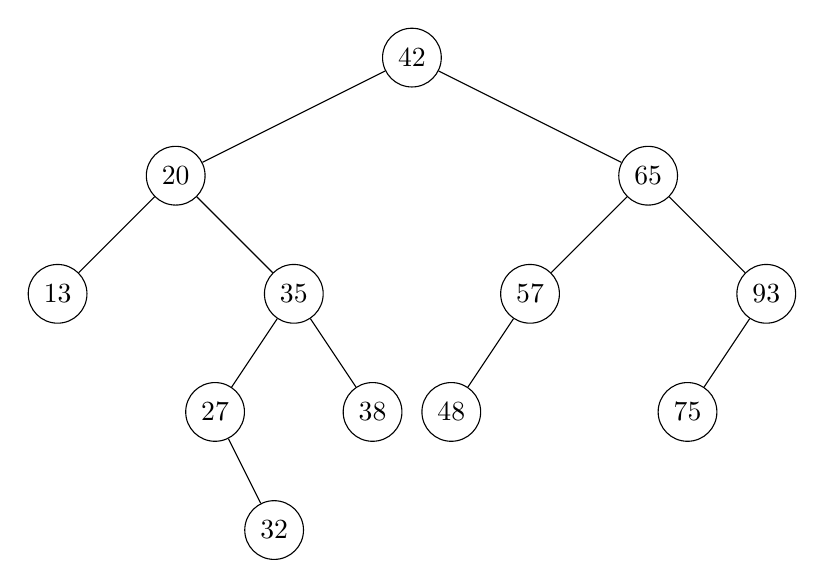
\begin{tikzpicture}[level/.style ={sibling distance=60mm/#1}]
              \node[circle,draw] (a) {42}
                child {node [circle,draw] (b) {20}
                  child {node [circle,draw] (c) {13}
                  }
                  child {node [circle, draw] (e) {35}
                    child {node [circle, draw] (f) {27}
                      child[missing] {node {}}
                      child {node [circle, draw] (m) {32}}
                    }
                    child {node [circle, draw] (g) {38}}
                  }
                }
                child {node [circle, draw] (h) {65}
                  child {node [circle, draw] (i) {57}
                    child {node [circle, draw] (j) {48}}
                    child[missing] {node {}}
                  }
                  child {node [circle, draw] (l) {93}
                    child {node [circle, draw] (m) {75}}
                    child[missing] {node {}}
                  }
                };
            \end{tikzpicture}
            \caption{Zwischenbaum: Baum B6 durch Einfügen von 32 in B1}
            \label{fig:baum}
          \end{figure}

          \begin{figure}[!h]
            \centering
            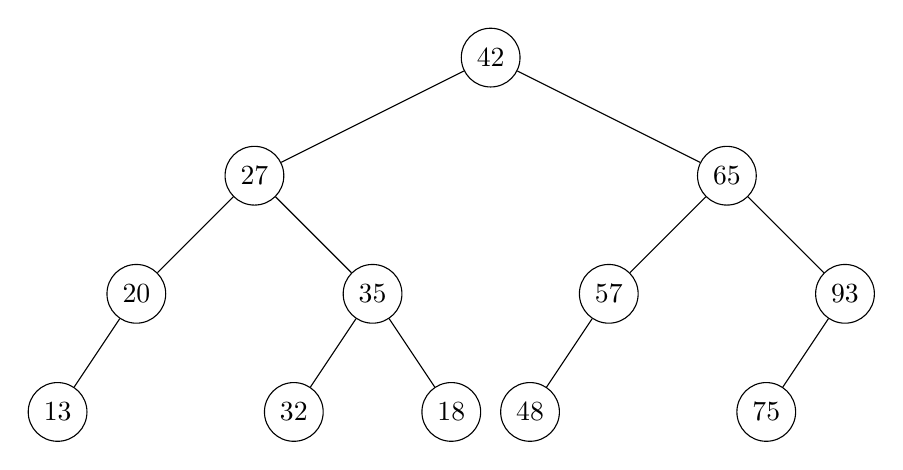
\begin{tikzpicture}[level/.style ={sibling distance=60mm/#1}]
              \node[circle,draw] (a) {42}
                child {node [circle,draw] (b) {27}
                  child {node [circle,draw] (c) {20}
                    child {node [circle, draw] (m) {13}}  
                    child[missing] {node {}}  
                  }
                  child {node [circle, draw] (e) {35}
                    child {node [circle, draw] (f) {32}}
                    child {node [circle, draw] (g) {18}}
                  }
                }
                child {node [circle, draw] (h) {65}
                  child {node [circle, draw] (i) {57}
                    child {node [circle, draw] (j) {48}}
                    child[missing] {node {}}
                  }
                  child {node [circle, draw] (l) {93}
                    child {node [circle, draw] (m) {75}}
                    child[missing] {node {}}
                  }
                };
            \end{tikzpicture}
            \caption{AVL-Baum: Baum B6 durch Einfügen von 32 in B1}
            \label{fig:baum}
          \end{figure}
      \end{enumerate}
  \end{enumerate}

\newpage
\setcounter{exnum}{4} % Nummer der Aufgabe
\exercise{Bonäre Suchbäume}

\begin{figure}[!h]
  \centering
  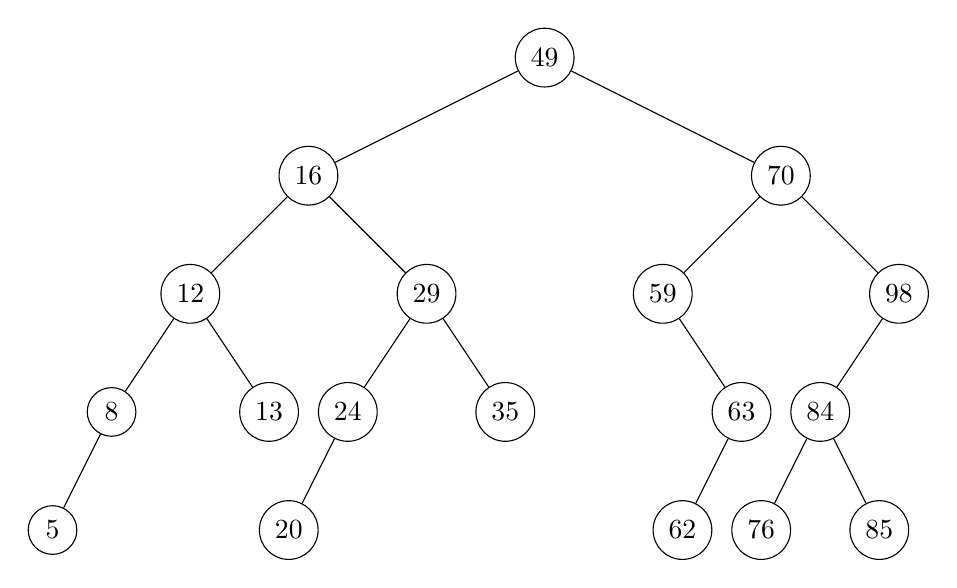
\begin{tikzpicture}[level/.style ={sibling distance=60mm/#1}]
    \node[circle,draw] (a) {49}
      child {node [circle,draw] (b) {16}
        child {node [circle,draw] (c) {12}
          child{node [circle, draw] (d) {8}
            child {node [circle, draw] (m) {5}}
            child[missing] {node {}}
          }
          child{node [circle, draw] (d) {13}}
        }
        child {node [circle, draw] (e) {29}
          child {node [circle, draw] (f) {24}
            child {node [circle, draw] (m) {20}}
            child[missing] {node {}}
          }
          child {node [circle, draw] (g) {35}}
        }
      }
      child {node [circle, draw] (h) {70}
        child {node [circle, draw] (i) {59}
          child[missing] {node {}}
          child {node [circle, draw] (j) {63}
            child {node [circle, draw] (m) {62}}
            child[missing] {node {}}
          }
        }
        child {node [circle, draw] (l) {98}
          child {node [circle, draw] (m) {84}
            child {node [circle, draw] (n) {76}}
            child {node [circle, draw] (p) {85}}
          }
          child[missing] {node {}}
        }
      };
  \end{tikzpicture}
  \caption{Suchbaum}
  \label{fig:baum}
\end{figure}
\end{document}
